The initial landing attempts were conducted as follows. A pilot manually hovered the drone over the landing pad in order to provide the drone with a view of the WhyCon marker. Visual acquisition of the marker was verified simply by ensuring that the gimbal was changing orientation to aim the camera at the landing pad. After visual acquisition was confirmed, the drone was placed from ``STABILIZE'' mode into ``GUIDED'' mode, enabling the landing controller to command the drone using positional targets.

The first attempts were made with the Jetson Nano drone (as shown in Figure \ref{fig:jetson_in_flight}), whose power issues prevented reliable visual acquisition of the landing pad. Although the drone was able to successfully hover and all components except for the Jetson Nano ran without problems, the landing attempts ultimately had to be delayed until these issues are fixed.

\begin{figure}
    \centering
    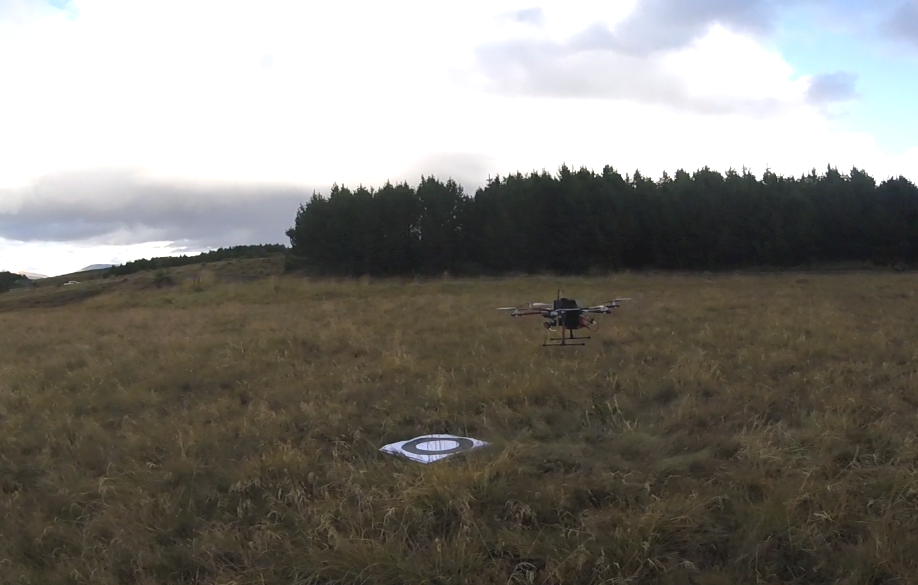
\includegraphics[width=0.75\textwidth]{images/drone_in_flight.png}
    \caption{The Jetson drone in flight.}
    \label{fig:jetson_in_flight}
\end{figure}

The next attempts were made with the Google Coral drone. This drone was able to successfully identify and track the landing pad in flight. Upon switching to ``GUIDED'' mode, the drone successfully approached the landing pad in the plane and decreased its height. However, because of a combination of factors, the final touchdown was not successful. First the region of allowable descent was too tight, meaning that the drone would have to land in an area defined by a 30cm radius. This by itself is not a problem, but becomes a problem because of the inaccuracies in pose estimation when the marker is viewed from extreme angles: the magnitude of the pose becomes smaller than in actuality, meaning that a small positional drift by the drone can be perceived as a prohibitively large positional drift. Essentially, the drone perceives itself as outside of the descent region and attempts to correct its horizontal position before descending. Moreover, there is another phenomenon at play called the ``ground effect.'' This occurs when the drone is close enough to the ground that the air pushed by the propellers bounces off the ground and produces a secondary thrust effect, changing the dynamics of the system \cite{ground_effect_article}. It is harder for the drone to maintain its position when it is close to the ground because of this extra turbulence. Therefore, although the drone successfully approached the landing pad, attained an acceptable horizontal position for landing, and descended to only about 5-10 centimeters from the ground, it never fully reached the ground autonomously.

All of these issues represent surmountable challenges only, and specifically \textit{not} prohibitive obstacles. They can be solved with iterative adjustment of the landing control policy and re-calibration of the WhyCon system, as well as possible filtering of the position of the landing pad. However, the limited time for a summer project means that this is not yet accomplished. It is part of our future work. So far, we have carried out 6 testing attempts, with multiple flights per attempt. These were conducted just east of Reykjavik.